\documentclass[12pt,a4paper]{book}
\usepackage[utf8]{inputenc}
\usepackage[french]{babel}
\usepackage[T1]{fontenc}
\usepackage{amsmath}
\usepackage{amsfonts}
\usepackage{amssymb}
\usepackage[left=2cm,right=2cm,top=2cm,bottom=2cm]{geometry}
\usepackage{algorithme}
\usepackage{siunitx}
\usepackage {titlesec}
\usepackage{tikz}
\usepackage{pgfplots}
\usepackage{graphicx}
\usepackage{fancyhdr}
\usepackage{sectsty}


\usepackage{arabtex}
\usepackage{utf8}

\pagestyle{fancy}



\titleformat{\chapter}[display]  
{\normalfont\huge\bfseries}{\chaptertitlename\ \thechapter}{0pt}{\Huge}  
\titlespacing{\chapter}{0pt}{-20pt}{40pt}  


\begin{document}
\let\cleardoublepage\clearpage
%\pagestyle {empty}
\frontmatter


%----------------------------------------------------------------------------------------
%	THESIS CONTENT
%----------------------------------------------------------------------------------------

%\lhead{\emph{Sommaire}} % Set the left side page header to "Contents"
\tableofcontents % Write out the Table of Contents

\clearpage % Start a new page

%----------------------------------------------------------------------------------------
%	CHAPTERS
%----------------------------------------------------------------------------------------

\mainmatter % Begin numeric (1,2,3...) page numbering

\setlength\parindent{24pt}

%\pagestyle {fancy}

%\renewcommand \headrulewidth {3pt}
%\fancyhead [L]{} % pour avoir le nom et numéro du chapitre en cours en haut à gauche dans l’entete.
%\renewcommand \footrulewidth {1pt}
%\fancyfoot [C]{\pageref }

%\fancyfoot [C]{\LaTeX :\\ \textbf {Page : \thepage /\pageref {LastPage}}}

\setcounter{page}{1}
\fancyhf{}
\renewcommand{\headrulewidth}{1pt}
\fancyfoot [C]{\thepage }


% Chapter 0
\chapter*{Introduction générale}

\label{Chapter0} % Change X to a consecutive number; for referencing this chapter elsewhere, use \ref{ChapterX}

\lhead{\emph{Introduction générale}} % Change X to a consecutive number; this is for the header on each page - perhaps a  shortened title



%------------------------------------------------------------------------------
%	INTRODUCTION GENERALE
%----------------------------------------------------------------------------------------

\paragraph*{}
Il est bien simple et évident pour nous, humains, de reconnaître ce que nous voyons instantanément.  Cependant, ce n'est pas aussi simple pour un ordinateur. Étant donné la puissance et la compléxité des traitements effectués par notre cerveau, il nous est très difficile de les analyser, et d'autant plus à les reproduire. 

\paragraph*{}
Si on prend en exemple la reconnaissance et la segmentation des textures qui sont aussi une partie du domaine du traitement d’images, nous nous retrouvons dans le paradoxe de l’étude d’une entité non défini mais parfaitement reconnaissable. Le fait de reconnaître un ciel bleu et le distinguer d’une rivière ou des roches tout au tour est élémentaire pour le cerveau humain et utilisé instinctivement par ce dernier. On peut aussi très facilement distinguer une table en plastique d’une table en bois. Cependant, la simple définition du  terme «\textit{texture}» reste ambiguë. 

\paragraph*{}
Comment pouvons nous donc traiter une entité indéfinie?

\paragraph*{}
La réponse se trouve dans les études statistiques sur les différentes relations qui existent entre les pixels qui forment une image.
Les chercheurs ont pu trouver différentes formules et caractéristiques afin de définir et segmenter les textures. La plupart du temps, l'étude s'intéresse surtout à la détection de motifs réguliers formant la texture, et cela en comparant chaque pixel avec la disposition de son entourage.

\paragraph*{}
La plupart des travaux fait dans ce domaine jusque là, visent à reconnaître une texture dans une image en ayant initialement une partie de cette première comme référence. Ceci est employé dans la recherche de motif déjà connu.

\paragraph*{}
Notre travail consiste à proposer une généralisation de ces méthodes afin de pouvoir l'implémenter dans des systèmes autonomes. Ces derniers doivent être capables d'extraire automatiquement les informations d'une image digitale. En d'autres termes, ils doivent pouvoir segmenter les différentes textures qu'on leur présente.\\


\paragraph*{}
Notre mémoire est organisé en trois chapitre. Nous présenterons dans le premier chapitre des généralités, des définitions et des notions de bases sur les méthodes utilisées dans notre travail. Dans le second chapitre nous introduirons en détails le principe de l'approche utilisée pour la segmentation des textures. Le troisième sera consacré à la présentation de notre application ainsi que les testes réalisés sur des images générées aléatoirement.

%----------------------------------------------------------------------------------------
% Chapter 1
\chapter{Généralités sur la segmentation de texture} % Main chapter title

\label{Chapter1} % Change X to a consecutive number; for referencing this chapter elsewhere, use \ref{ChapterX}

\lhead{Chapitre 1. \emph{Généralités sur la segmentation de texture}} % Change X to a consecutive number; this is for the header on each page - perhaps a shortened title


\section{introduction}

Dans ce chapitre, nous examinerons les différentes définitions de texture proposés par plusieurs chercheurs du domaine. Puis nous verrons les notions de bases du traitement d'images et un apperçu de ses domaines d'utilisation . Nous découvrirons enfin, plus en détails, la méthodes que nous avons utilisés pour caractériser une textures.

\section{Définition de la texture}

\indent Certaines définitions de la texture ont été sélectionées et regroupées dans un catalogue par Coggins [COG 82]. On peut en citer quelques exemples:\\


\begin{itemize}
\item \indent "Nous pouvons considérer une texture comme ce qui constitue une région macroscopique. Sa structure est simplement attribuable aux motifs répétitifs dans lesquels des éléments ou des primitives sont disposées selon une règle de placement."[Tam et.al 78] \\ 

\item \indent "La texture est défini pour nos fins comme un attribut d'un domaine n'ayant aucune composante qui apparaissent dénombrable. Les relations de phase entre les composants ne sont donc pas apparentes. Le terrain ne devrait pas contenir un gradient évident. Le but de cette définition est d'attirer l'attention de l'observateur sur les propriétés globales de l'affichage -. C'est à dire sa "rudesse" globale "bosselage", ou "finesse". Physiquement, les modèles innombrables (apériodiques) sont générés par stochastique par opposition de processus déterministes. A la perception, cependant, l'ensemble des motifs sans composants énumérables évidentes comprendra de nombreux (et même périodique) textures déterministes."[Ric et.al 74]\\

\item \indent "La texture est une notion apparemment paradoxale. D'une part, elle est couramment utilisée dans le traitement de l'information visuelle, surtout pour des raisons pratiques de classification. D'autre part, personne n'a réussi à produire une définition communément acceptée de la texture. La résolution de ce paradoxe, dépendra d'un modèle plus riche, plus développé pour le début de traitement de l'information visuelle, un aspect central de ce qui sera un systèmes représentatif à différents niveaux d'abstraction. Ces niveaux vont probablement inclure
-----------------------------------------
 intensités actuels au fond et progresseront à travers des pointes et des descripteurs d’orientation vers la surface, et peut-être des descripteurs volumétriques. Compte tenu de ces structures multi-niveaux, il semble clair qu'ils doivent être inclus dans la définition, et dans le calcul des  descripteurs de la texture."[Zuc et.al 81]\\

\item \indent "La notion de texture semble dépendre de trois ingrédients: (1) un certains « ordre » local répété sur une région qui est grande par rapport à la taille de l'ordre, (2) l'ordre consiste en l'arrangement non aléatoire de pièces élémentaires et (3) les parties sont des entités plus ou moins uniformes ayant approximativement les mêmes dimensions partout dans la région texturée."[Haw 69]\\\\
\end{itemize}

\begin{figure}[htbp]
\centering
\begin{tabular}{cc}
\centering
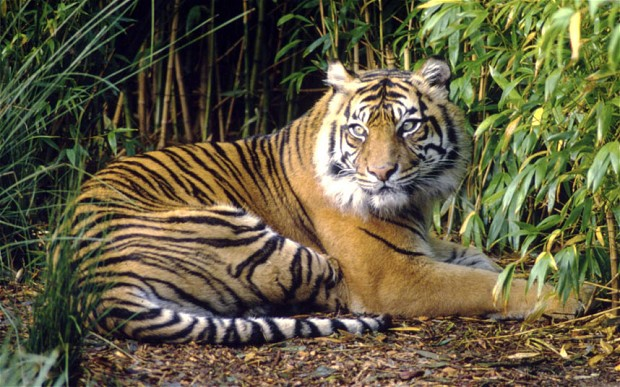
\includegraphics[width=6cm, height=4.5cm]{Figures/chap1/tigre.jpg}
&
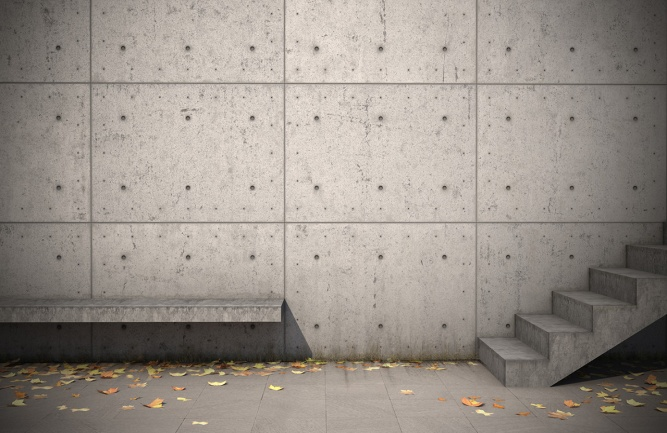
\includegraphics[width=6cm, height=4.5cm]{Figures/chap1/beton.jpg}\\

(a)
 &
(b)

\end{tabular}
\caption[textureDif]{Différentes textures\\}
\end{figure}


Quelques paramètres essentiels sont à prendre en compte dans l’étude des textures. Si on prend par exemple la photo d’une forêt, on pourra distinguer la terre comme texture,  l’ensemble des feuille d’un arbre comme une autre, mais encore la peau d’un tigre [Figure 1.1](a).\\

Si on prend par contre une prise aérienne de cette même forêt, on pourra considérer le tout comme une seule texture qui se différenciera de la texture formée par les bâtiments d’un village par exemple. 
Aussi, le voisinage d’une texture joue un grand rôle dans l’interprétation de cette dernière. Une couche de béton par exemple seule peut avoir plusieurs interprétations, elle peut être une partie d’un mur,  un banc, le sol ou  bien des marches d’escalier [Figure 1.1](b).\\

Notons aussi que certaines structures ont une dynamique importante au fil du temps qui fait varier leur apparence. Par exemple un ciel bleu avec quelques nuages (le vent fera constamment varier la forme des nuages).\\ 

%------------------------------------------------
%-------- [1] SEGMENTATION D'IMAGES -------------
%------------------------------------------------


\section{Segmentation d’images}

\indent Dans le traitement d’image, une des plus grandes préoccupations est la segmentation d’images. C’est, comme son nom l’indique, le processus de partitionnement d’image digitale en différentes parties et ce, pour simplifier la « compréhension »  de cette dernière par la machine, et la rendre plus facilement analysable.\\

Le principe est de reconnaître des objets ou des frontières. Le but étant de donner une signification aux pixels de l’image. Elle est généralement utilisée dans:.\\

\begin{itemize}
\item La vision artificielle [Figure 1.2](a)\\
\item \indent L’imagerie médicale [Figure 1.2](b)\\
\item \indent La reconnaissance faciale [Figure 1.2](c)\\
\item \indent La reconnaissance d'empreintes digitales [Figure 1.2](d)\\
\item \indent La détection de piétons [Figure 1.2](e)\\
\item \indent La vidéo surveillance [Figure 1.2](f)\\
\item \indent Localiser des objets dans des images satellitaires [Figure 1.2](g)\\
\end{itemize}

\begin{figure}[h]
\centering

\begin{tabular}{cccc}

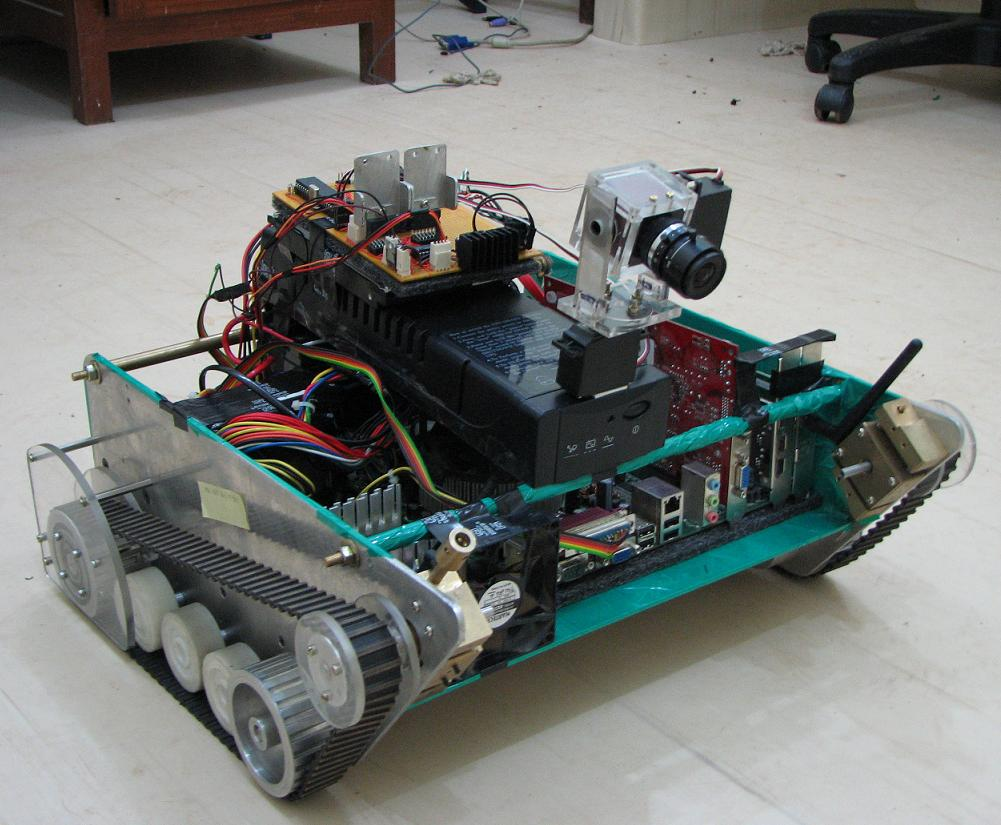
\includegraphics[width=5.5cm, height=3.5cm]{Figures/chap1/VisionArtificielle1.jpg}
&
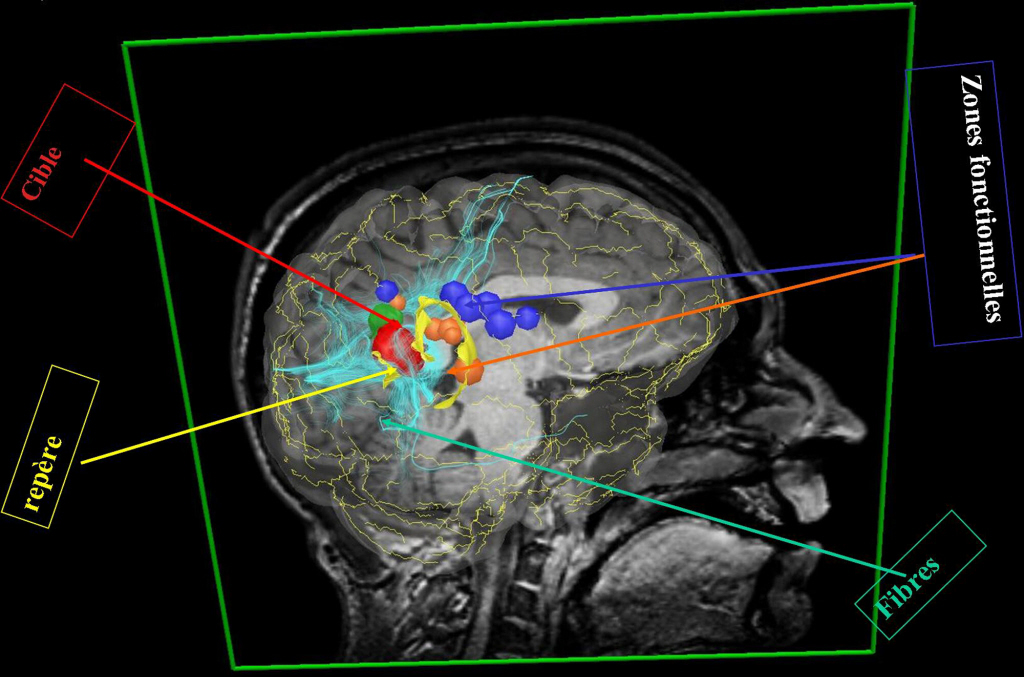
\includegraphics[width=5.5cm, height=3.5cm]{Figures/chap1/ImagerieMedical.jpeg}\\
(a) & (b)\\\\

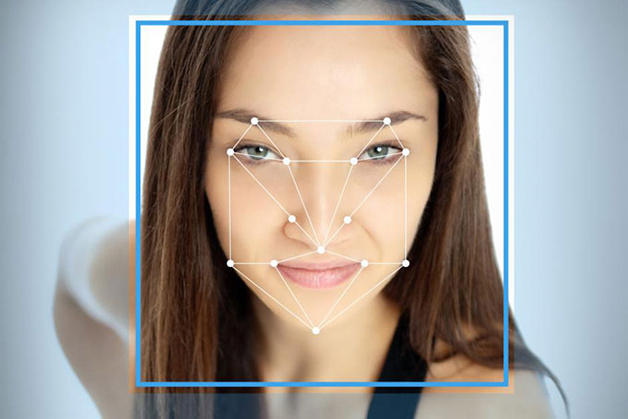
\includegraphics[width=5.5cm, height=3.5cm]{Figures/chap1/reconaissanceFacial.jpg}
&

\includegraphics[width=5.5cm, height=3.5cm]{Figures/chap1/empreinteDigitale.jpeg}\\
(c) & (d)\\\\

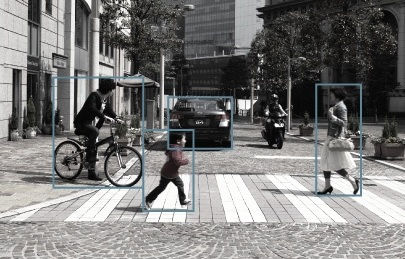
\includegraphics[width=5.5cm, height=3.5cm]{Figures/chap1/DetectionPieton.png}
&
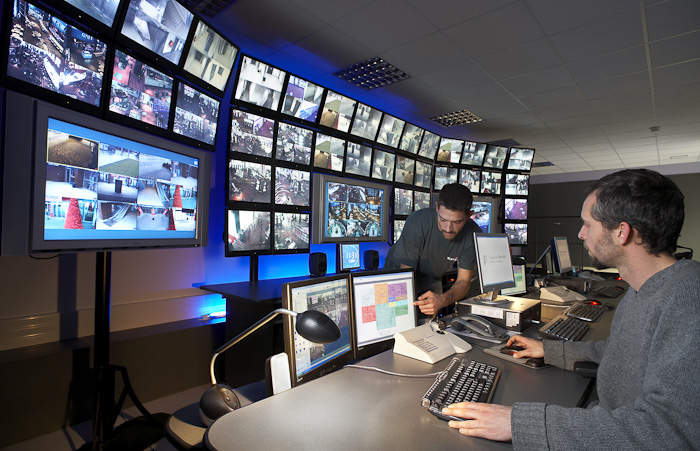
\includegraphics[width=5.5cm, height=3.5cm]{Figures/chap1/videoSurveil.jpeg}\\
(e) & (f)\\\\

\multicolumn{2}{c}{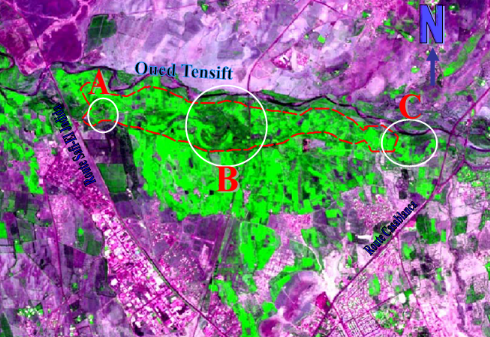
\includegraphics[width=5.5cm, height=3.5cm]{Figures/chap1/Satellite.png}}\\
\multicolumn{2}{c}{(g)}\\

\end{tabular}
\caption[TraitementImage]{La segmentation d'images}

\end{figure}


%------------------------------------------------
%------- [2] LES APPROCHES ANALYTIQUES ----------
%------------------------------------------------

\section{Les approches analytiques}

\indent On retrouve principalement quatre (4) approches analytiques de texture qui sont [MAT et STR 98]:\\
\begin{itemize}
\item \textit{Approche structurelle (ou fréquentielle)}: Ces méthodes supposent que les textures sont formées d’éléments structurants de base. L’idée générale de ces méthodes est une recherche et une description des éléments structurants suivie d’une étude de la répartition spatiale de ces derniers [MAJ 09].\\

\item \textit{Approche modèle} : Elle se repose sur l’utilisation de fractals et de modèles stochastique.\\

\item \textit{Approche transformée (méthodes de traitement du signale)} : Des recherches de  psychophysique ont démontrés que le cerveau humain fait une analyse de fréquence des images.\\ 

\item \textit{Approche statistique} : Ici, la texture est reconnu en utilisant des caractéristique tel que les "\textit{Motifs Binaires Locaux}"  en se basant sur distribution des niveaux de gris dans l’image, et c’est sur quoi sera basée notre approche.\\
\end{itemize}

L’utilisation de ces approches diffère selon le type de texture. Ces dernières se regroupent en trois différentes catégories : structurelles, aléatoires et directionnelles.


\subsection{Textures structurelles}

\begin{figure}[htbp]
\centering
\begin{tabular}{cc}
\centering

	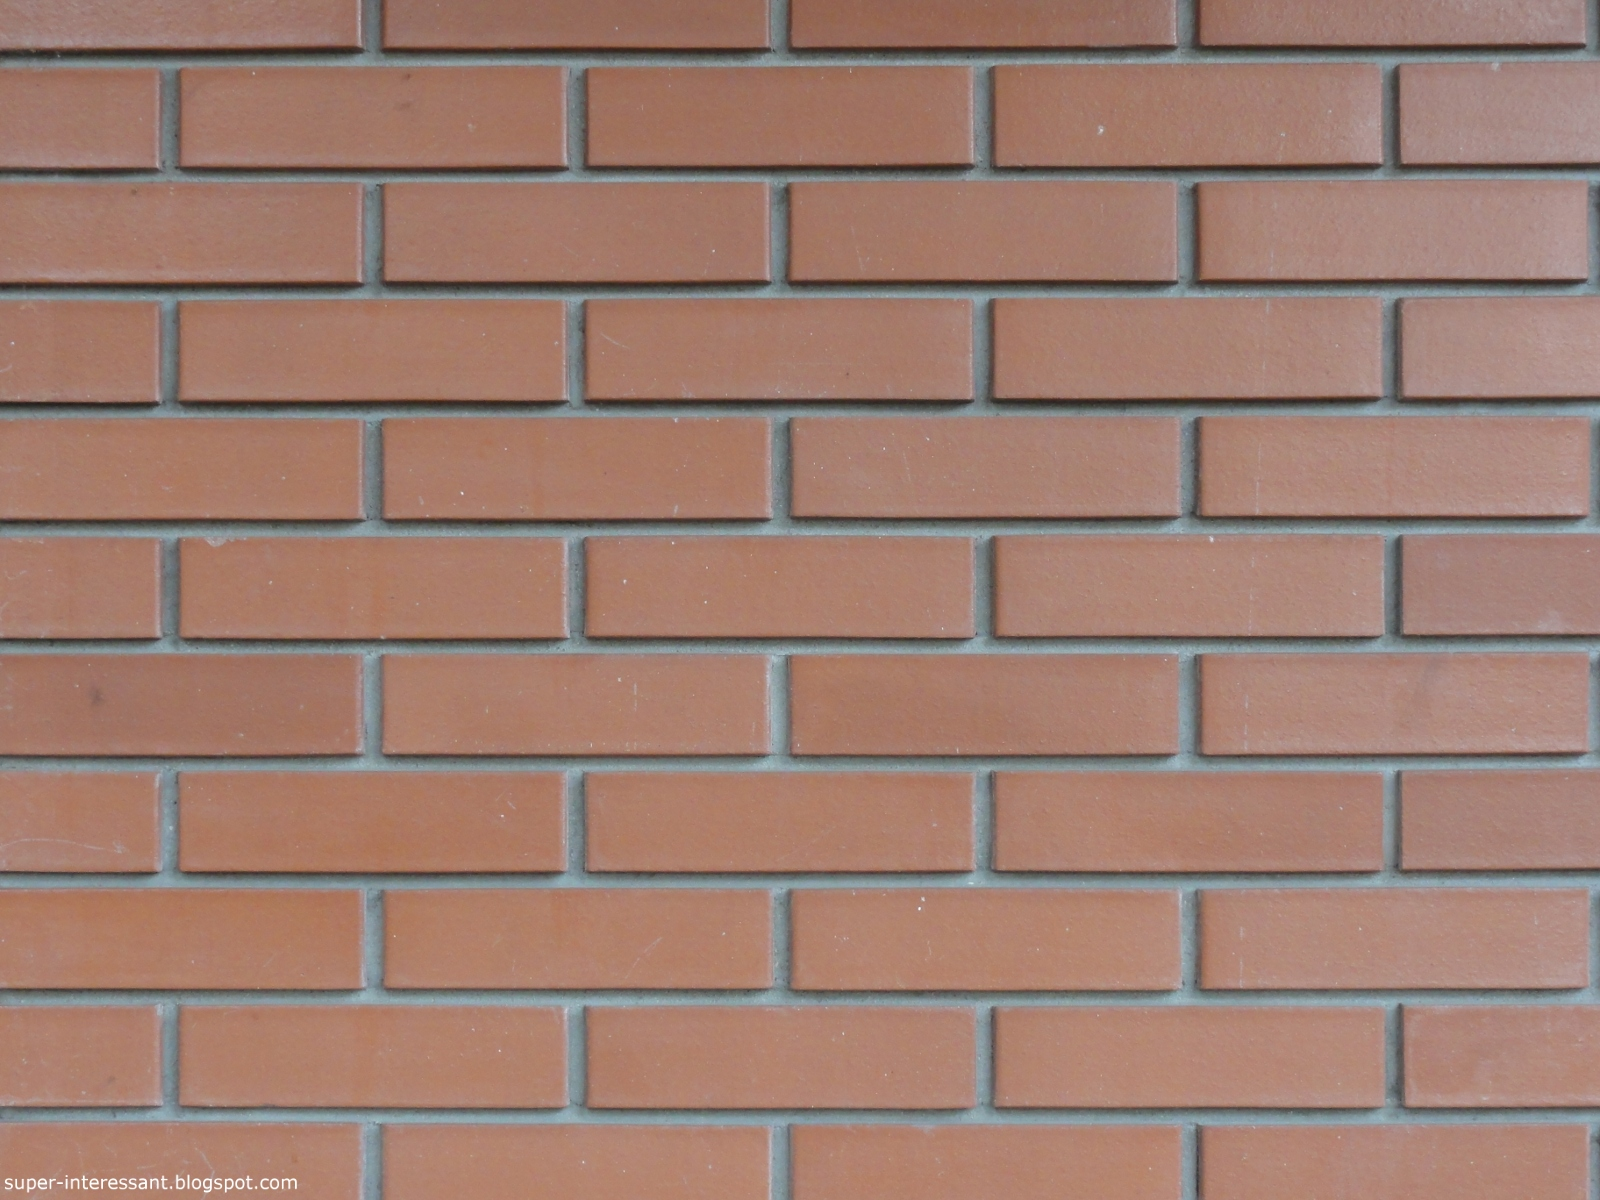
\includegraphics[width=5cm,height=3cm]{Figures/chap1/mur.jpg}	
&
	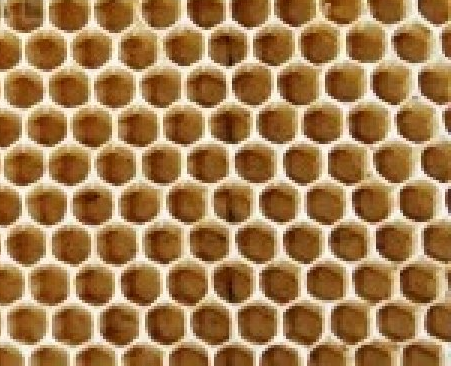
\includegraphics[width=5cm,height=3cm]{Figures/chap1/beehive.png}	

\end{tabular}
	\caption[textureStruc]{Textures structurelles (périodique)}
\label{fig:textureStruc}
\end{figure}


\indent La figure 1.3 présente un premier type de textures dites structurelles.
On les appelle ainsi car on peut les considérer comme étant la répartition spatiale de motifs élémentaires de base dans différentes directions de l’espace tout en respectant une certaine règle de placement. En effet, on s’aperçoit que la première représente un mur de brique, elle est composée d’un ensemble d’éléments de base (les briques) disposés relativement régulièrement de manière horizontale. La deuxième texture est aussi composée de motifs de base alvéolés agencés d’une manière particulière les uns à côté des autres [MAJ 09].
Cette catégorie de textures a engendré des méthodes d’analyse dites structurelles.

\subsection{Textures aléatoires}

\begin{figure}[H]
\centering
\begin{tabular}{cc}
\centering

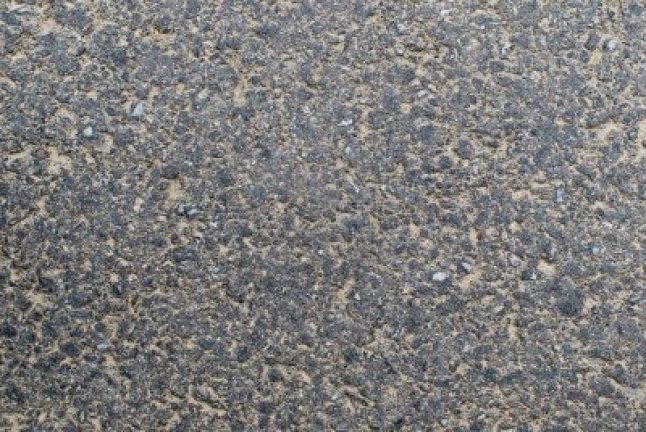
\includegraphics[width=5cm,]{Figures/chap1/aleatoire1.png}
&

\includegraphics[width=5cm,]{Figures/chap1/aleatoire2.png}\\

\end{tabular}
\caption[textureAleat]{Textures aléatoires}
\end{figure}


\indent Le deuxième type de textures est illustré dans la figure 1.4. Contrairement au premier type de texture, celles-ci ont un aspect anarchique tout en restant globalement homogènes. Ces textures ne peuvent pas être décomposé en des motifs de base se répétant spatialement. On les appelle des textures aléatoires.
Cette catégorie a fourni d’autres travaux de recherches plutôt fondés sur des méthodes d’analyse statistique [MAJ 09].

\subsection{Textures directionnelles}

\begin{figure}[htbp]
\centering
\begin{tabular}{ccc}
\centering
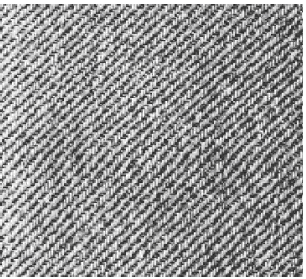
\includegraphics[width=5cm,]{Figures/chap1/direction.png}
&
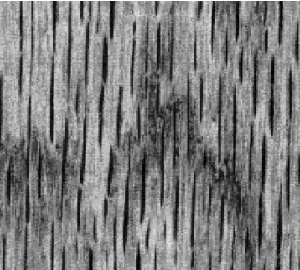
\includegraphics[width=5cm,]{Figures/chap1/directionel1.png}
&

\includegraphics[width=3.5cm,]{Figures/chap1/directionel2.png}\\

\end{tabular}
\caption[textureDirex]{Textures directionnelles}
\end{figure}              


\indent Les textures directionnelles [Figure 1.5] ne sont pas forcément aléatoires et ne présentent pas d’éléments structurants de base.
On peut les décrire de manière générale comme étant des textures  présentant des structures orientées selon une direction privilégiée.
Les textures directionnelles se caractérisent soit par leur orientation globale, soit par un champ d’orientations locales. par exemple la texture de gauche de la figure 1.5 laisse apparaître des lignes obliques, et celle au milieu possède des lignes verticales.
Dans les textures directionnelles réelles, le champ d’orientation n’est en effet pas toujours uniforme comme la texture de droite de la figure 1.5.


\indent Les différentes catégories de textures qui ont été présenté nous montrent qu’il est difficile de donner une définition "universelle" de la texture. Cependant, on peut décrire le type de la texture selon la distribution et les relations entre les pixels qui la forment.\\

\indent Nous allons nous approfondir sur l’approche statistique étant donné qu’elle sera celle qu’on implémentera dans nôtre étude.
Plus précisément, nous étudirons la méthode suivante dite \textbf{motif binaire local}.


%------------------------------------------------
%------ [3] MOTIFS BINAIRE LOCAL (LBP) ----------
%------------------------------------------------

\section{Motif binaire local (LBP-Local Binary Pattern)}
\indent Cette caractéristique a été premièrement évoqué par Harwood [Har et.al 93] et a été utilisé après par Ojala et Pietikinen [Oja et.al 96, Oja and Pie 99].
La caractéristique LBP présente un énorme avantage grâce à sa simplicité de calcul et sa robustesse dans la détection de textures. Elle permet de décrire la texture suivant la configuration 

 locale des pixels.\\ 
\indent Le principe de calcul de la LBP basique (\textit{Basic Local Binary Pattern}) réalisé par Ojala [Oja et.al 02] est de comparer un pixel se trouvant au centre avec ces 8 voisins comme le montre la figure suivante :

\begin{figure}[H]
\centering
\begin{tabular}{ccc}
\centering

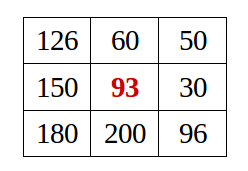
\includegraphics[width=5cm,height=3cm]{Figures/chap1/matrice1.png}
&
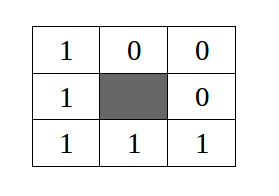
\includegraphics[width=5cm,height=3cm]{Figures/chap1/matrice2.png}
&
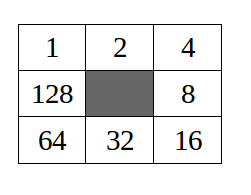
\includegraphics[width=5cm,height=3cm]{Figures/chap1/matrice3.png}\\
(a) & (b) & (c)\\
\end{tabular}
\caption[CalcMotif]{Calcul du motif binaire}
\end{figure}

\indent La matrice \textit{I} de la figure 1.6 (a) représente le niveau de gris d'un pixel au centre et de ses huit voisins. La matrice \textit{M} du \textit{motif} qui est représenté dans la figure 1.6 (b) est calculé comme suit :
$$M(i,j) = \left\{
\begin{array}{c c c}      
    1 & si & I(i,j)\geqslant g_{c}\\
    0 & sinon & 
\end{array}\right. $$
Où $I(i,j)$ est la valeur du niveau de gris des huit voisins, et $g_{c}$ qui est le niveau de gris du pixel central (en rouge), le résultat est alors affecté sous format binaire dans les $M(i,j)$.\\
En lisant les valeurs de $M(i,j)$ en commençant de la case qui se trouve en haut à gauche et en suivant l'ordre de rotation de l'aiguille d'une montre, on obtient le motif binaire \textit{m} suivant :

$$ m = 10001111 $$

Ce résultat sera ensuite converti en décimal et cela en multipliant chaque chiffre par les valeurs $P(i,j)$ case par case de la matrice de Poids de la [Figure 1.6](c), ce qui nous donne la valeur LBP du niveau de gris du pixel central qui est :

$$ LBP = 128+8+4+2+1 = 143 $$

La figure suivante montre la transformation LBP d'une image :

\begin{figure}[H]
	\centering
	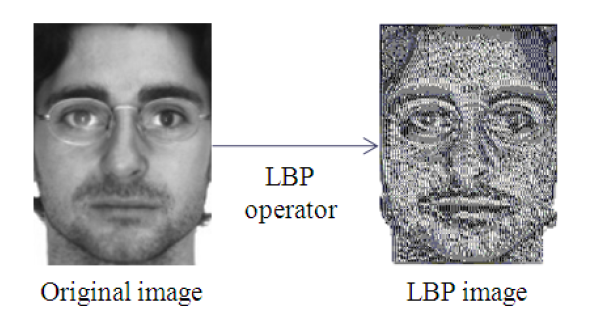
\includegraphics[width=9cm,]{Figures/chap1/transLBP.png}		
	\caption[transLBP]{Transformation LBP de l'image}
\end{figure}	


\indent Ojala [Oja et.al 02] a aussi définie une valeur "\textit{U}" qu'on appellera valeur de «\textit{transition}» qui sera égale au nombre de transitions de 0 vers 1 et de 1 vers 0 qu'on trouve dans la valeur du «\textit{motif binaire}» comme suit :\\

\begin{figure}[H]
	\centering
	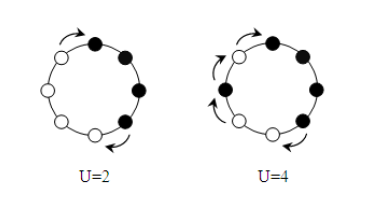
\includegraphics[width=8cm]{Figures/chap1/extractU.png}		
	\caption[extractU]{ Extraction du nombre U à partir du motif}
\end{figure}	

\indent En réalité, tous les «\textit{motifs}» (256) ne sont pas importants pour décrire une texture.
D'apres T. Menp [Men et.al 00], les motifs qui ont un nombre de transition $U=2$ et $U=0$, et qui sont appelés «\textit{uniform patterns}», représentent une information relative à des motifs réguliers d'une image, autrement dit une texture. Et donc, certaines zones d'intérêt tels des coins ou des bords peuvent être détectées par ce descripteur.
Ces motifs sont aussi plus résistants aux transformations géométriques telle que la rotation.
L’utilisation des 58 «\textit{uniform patterns}» suivants a été proposé :

\begin{figure}[H]
	\centering
	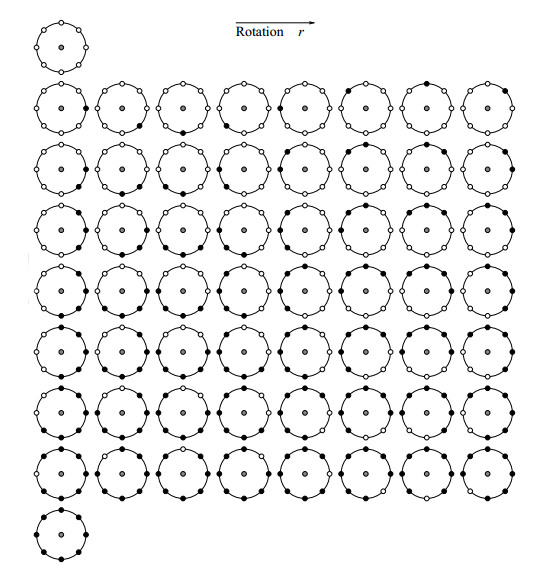
\includegraphics[height = 12cm]{Figures/chap1/uniforme.png}		
	\caption[uniforme]{ Les «\textit{uniform patterns}».}
\end{figure}	

\indent Pour étudier l’uniformité d'une texture, on construit un histogramme qui est composé de 59 valeurs qui sont les 58 «\textit{uniform patterns}» définis plus haut, plus une dernière valeur regroupant tous les «\textit{non uniform patterns}».\\

\begin{figure}[H]
\centering
\begin{tabular}{cc}
\centering

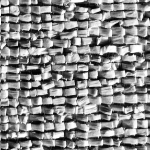
\includegraphics[width=3cm,height=6cm]{Figures/chap1/in1.png}
&
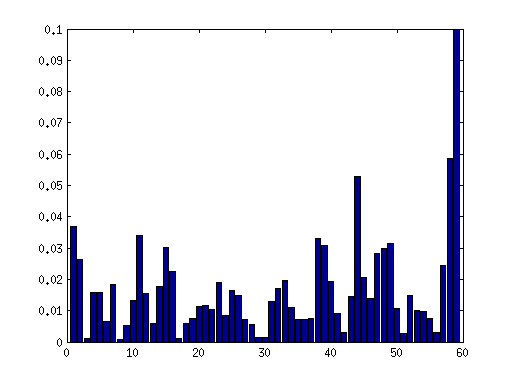
\includegraphics[width=6cm,height=6cm]{Figures/chap1/histo1.png}\\
(a) & (b) \\
\end{tabular}
\caption[histo]{Une texture et son histogramme LBP }
\end{figure}


\indent On compare deux histogrammes LBP de deux textures selon un pourcentage de ressemblance qu'on appellera «\textit{seuil}» ou encore «\textit{Threshold}».On pourra ainsi dire si ces deux textures représentent la même texture ou bien non grâce à cette valeur. 

\indent La caractéristique LBP qui utilisent ce genre d'histogramme est noté en tant que $LBP^{u2}$. Cette notation est du au fait qu'elle se base sur les «\textit{uniform patterns}» qui ont un $U \leq 2$, par la suite, on notera la $LBP^{u2}$ en tant que LBP.

\subsection{LBP et le niveau de gris}
\indent L'un des avantages de la LBP est sa robustesse vis à vis du changements monotones du niveau de gris. Ainsi, si on augmente ou diminue le niveau de gris de chaque pixel d'une image d'une même valeur $x$, cela n'affectera pas l'histogramme LBP créée. Cet avantage réside dans la manière de calcul du nouveau niveau de gris LBP d'un pixel.\\
\indent Soit un pixel $P$ qui va avoir une nouvelle valeur modifié par $x$, il sera comparé avec ses voisins $V_{i}$ (sachant que ses voisins sont aussi affecté par la valeur $x$) et on sait que :
\begin{center}
si $P > V_{i}$ alors $P + x > V_{i} + x $
\end{center}
\indent Et comme la comparaison n'a pas changé, alors la nouvelle valeur de niveau de gris du pixel centrale restera toujours la même, comme le montre la figure 1.10.\

\begin{figure}[H]
\centering
\begin{tabular}{cc}
\centering

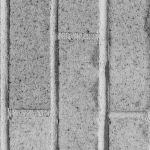
\includegraphics[width=3cm]{Figures/chap1/p1.png}
&
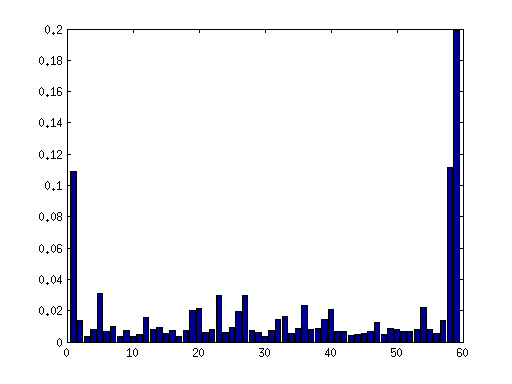
\includegraphics[width=6cm]{Figures/chap1/histcomp1.png}\\

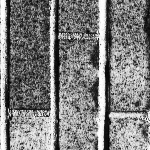
\includegraphics[width=3cm]{Figures/chap1/p2.png}
&
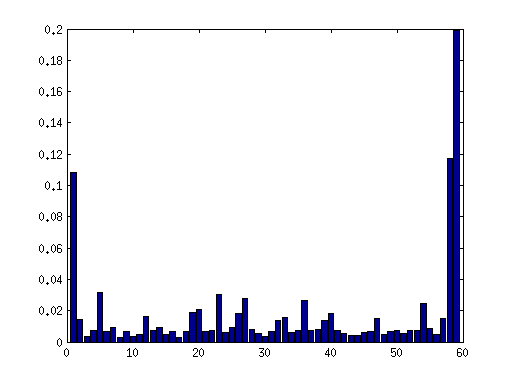
\includegraphics[width=6cm]{Figures/chap1/histcomp2.png}\\
\end{tabular}
\caption[comp]{Histogramme d'une texture subissant un changement monotone du niveau de gris}
\end{figure}


\subsection{Variantes de la LBP}
\indent Il existe d'autres variantes de la LBP qui divergent selon le nombre $P$ de voisins dans un rayon $R$, comme le montre la figure 1.11.\\
 
\begin{figure}[H]
\centering
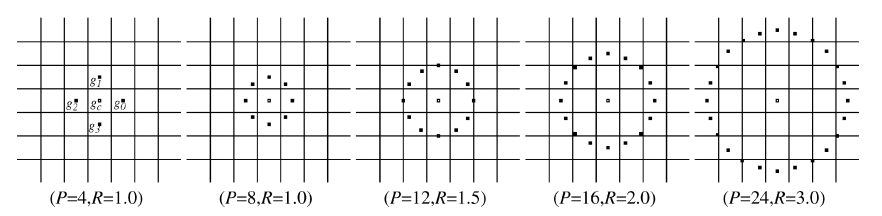
\includegraphics[width=15cm]{Figures/chap1/lbpvariantes.png}
\caption[lbpvar]{Variantes de la LBP}
\end{figure}

\indent Il a été noté que dans la LBP Basique ($P=8$ et $R=1$), le taux des «\textit{uniform patterns}» est presque de 90\%, alors que pour la LBP(16,2) ($P=16$ et $R=2$) ce taux ne dépassait pas les 70\%.[Oja et.al 02]
De ce fait, on se basera sur la LBP Basique qui offre une meilleure détection des textures.


\section{Conclusion}

\indent Dans ce chapitre nous avons décris la texture et ses différents types. Nous constatons que malgré le fait qu'il n'existe à priori toujours pas de définition universelle de la texture, les méthodes de description structurelles restent largement les plus utilisés.\\
\indent Nous avons présenté le \textbf{Motif binaire local} qui est une caractéristique très populaire et récemment employée pour détecter des personnes et dans la reconnaissance faciale.
Dans le chapitre suivant, nous allons parler de son utilité dans notre travail.

% Chapter Template
\chapter{Conception} % Main chapter title

\label{Chapter2} % Change X to a consecutive number; for referencing this chapter elsewhere, use \ref{ChapterX}

\lhead{Chapitre 2. \emph{Conception}} % Change X to a consecutive number; this is for the header on each page - perhaps a shortened title

%----------------------------------------------------------------------------------------
%	SECTION 1
%----------------------------------------------------------------------------------------

\section{Introduction}

Nous présentons dans ce chapitre notre approche qui se base sur la méthode de segmentation dynamique. 
Nous décrirons cette méthode ou, plus précisément, nous nous intéresserons à son architecture de découpage que nous exploiterons dans notre algorithme.
Nous terminons avec des essais de quelques variantes.

\section{Vue global de notre approche}
La méthode LBP offre effectivement un excelent outil pour caractériser une texture. Cependant, son role s'arrête la. Pour pouvoir détecter efficacement les textures, il nous faudra appliquer un algorithme de ségmentation. Nous avons porté notre choix sur l'algorithme de segmentation dynamique [HAM et.al 13] qui forme une étape primordiale de notre travail de détection. Il se nome de la sorte car il se base sur des tailles de ségments variantes (nous expliquerons dans ce qui suit notre choix). \\

Cependant cette méthode ne permet que de chercher une unique texture qui est connue déjà à l'avance. Notre méthode présente alors une généralisation qui permet de segmenter l'image et détecter toutes ses textures, et ce, en ayant aucune information au préalable, à part l'image elle même.\\

Notre méthode a pour but de détecter chaque texture dans les différents endroits où elle est présente dans une image, sans affecter les surfaces qu'occupent les autres textures. On représente cette détection en coloriant avec une couleur unique les surfaces qui contiennent une même texture.\\

Nous fixons une taille d'échantillon "\textit{t}". Nous prendrons comme premier lieu un carré de cette taille au point (0px,0px) qui contient une première texture, et nous chercherons des ségments similaire. Nous colorions tous les ségments de la même couleur "\textit{C}". Ensuite, nous feront de même pour le prochain carré de taille "\textit{t}" non colorié.\\

Plusieurs résultats très satisfaisants ont pu être obtenus avec cette approche, et différentes variantes de notre méthode ont été appliqué.

%----------------------------------------------------------------------------------------
%	SECTION 2
%----------------------------------------------------------------------------------------

\section{Méthode de découpage}

\subsection{Définition}
\indent Une méthode de découpage est une opération visant à rassembler des pixels entre eux suivant des critères pré-définis. Dans notre cas, les critères de similitudes seront basés sur la ressemblance des textures, définie elle par les paramètres de la méthode LBP (I.4.B).\\

\subsection{Algorithme de découpage dynamique}
\indent L'algorithme sur lequel nous allons nous baser est décrit dans l'algorithme 1 [HAM et.al 13].
Nous nous basons sur celui-ci pour notre méthode de généralisation. Nous supprimons, le test de ressemblance à la texture de référence [Algorithme 1 - 4.c] pour sauvegarder tous les carrés générés.\\
\indent Nous supprimons cependant la phase de coloriage dans le test (6) [Algorithme 1 - 6] pour la remplacer par un \textit{return} qui nous retournera le tableau de tout les carrées sauvegardés.

Le processus de division est expliqué dans la figure suivante. [Figure 2.1]

\indent Nous avons choisi d'appliquer cet algorithme dans le but de proposer une solution de généralisation pour la recherche et la détection de plusieurs textures différentes qui sont présentes dans une image, car son aspect dynamique lui offre une bonne robustesse dont on peut citer :\\

\begin{itemize}
\item Des carrés de tailles différentes peuvent être extraits et analysés, grâce à leurs tailles dynamiques. L'ensemble comparé avec la fenêtre principale serait donc très riche et varié\\

\item Différentes formes hormis les carrés et différents points de convergence peuvent être considérés. Par conséquent, différentes configurations peuvent être étudiées.\\

\item L'indépendance entre l'architecture proposée et la méthode d'extraction des caractéristiques est le principal avantage de notre approche. Ce qui permet à cette méthode de s'adapter à différents cas d'utilisations.\\

\end{itemize}

%-------------- DEBUT : DECOUPAGE DYNAMIQUE -------------
\label{Algorithme de découpage dynamique}
\begin{algorithme}[H]
\caption{Algorithme de découpage dynamique}
\Function{Square dynamic decomposition system}
{\textit{img} : \textbf{image},\textit{textureRef} : \textbf{image}}{void}
{

1 Choose the converging point\textit{a}.\\
2  Consider the main window\\
3  Generate as many windows as possible(with the same size of MW)\\

4 \For { each window }
{
		\begin{itemize}
			\item[a] Apply the feature extraction method (LBP method);
			\item[b] Calculate the feature vector (LBP histogram);
			\item[c] Calculate the similarity Sim between the window’s feature with the sought texture feature
 			
		\end{itemize}\\

		d \If {\textit{Sim} is above the threshold}{ 
			Save the window’s position and its feature vector V
		}
}

5 Reduce the size of MW by the distance \textit{d}\\
6 \IfThenElse { the size of MW is below the minimum size }
	{
		Color the saved windows and terminate the process
	}
	{
		Goto step \textbf{3}
	}
}
\end{algorithme}

%-------------- FIN : DECOUPAGE DYNAMIQUE -------------

%----------------------------------------------------------------------------------------
%	SECTION 3
%----------------------------------------------------------------------------------------


\begin{figure}[H]
	\centering
		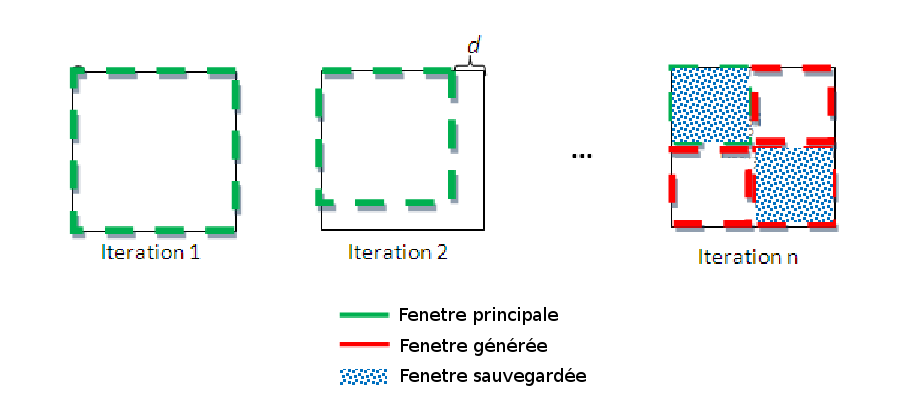
\includegraphics[width=14cm,]{Figures/chap2/1.png}
		
	\caption[division]{Processus de division.}
	\label{fig:division}
\end{figure}

\section{Généralisation de la méthode de recherches dynamique}

\indent Nous allons maintenant aborder tous les détails de notre approche de généralisation de la méthode cité ci-dessus.\\

\indent L'objectif étant de développer une méthode automatique de détection de toutes les textures présentes dans une image donnée, tout en minimisant au plus l'intervention de l'utilisateur. Chaque texture sera coloriée d'une couleur aléatoire et unique.

\subsection{Algorithme de généralisation}


%-------------- DEBUT : ALGORITHME DE GENERALISATION -------------
\label{Algorithme de généralisation}
\begin{algorithme}[H]
\caption{Generalization Algorithm}
\Function{Generalization Algorithm}
{\textit{img} : \textbf{image}}{void}
{
1 Constructing a blanc image with the same dimensions as \textit{img}\\
2 Applying the Square Dynamic Decomposition System without colouring \\
3 Save the result in a file\\
4 Set up a minimal size \textit{t} and a \textit{treshold}.\\
5 \While{ White window of dimension \textit{t} exists}
{
	a Brows the image from right to left, and from top to bottom, and extract the first white window
	\textit{Ref} with the dimension \textit{t} \\
	b Calculate the LBP histogram of \textit{Ref}\\
		
	c \For {each square}
		{
			calculate the resemblance \textit{Resmb} of the LBP histogram of the square with \textit{Ref}'s histogram

			\If{$Resmb > treshold$}{ 
				Colour the correspondent surface in the blanc image. 
				}
		}

}
}
\end{algorithme}

%-------------- FIN : ALGORITHME DE GENERALISATION -------------

\subsection{Interprétation de l'algorithme}

\indent Dans un premier lieu, nous nous contenterons d'appliquer l'algorithme sur des images simples.\\
Une image blanche \textit{IB} de même taille que l'image à découper est générée [Figure 2.2]. C'est cette première qui sera coloriée progressivement et rendu comme résultat finale de l'opération.

\begin{figure}[H]
	\centering
		
\includegraphics[width=14cm,]{Figures/chap2/2.png}
		
	\caption[initialisation]{Initialisation.}
	\label{fig:division}
\end{figure}

\indent L'algorithme de découpage présenté précédement est appliqué. Ce dernier nous retournera un ensemble de carrés que nous allons sauvegarder dans un fichier. La sauvegarde contiendra les coordonnées de l’extrémité initiale du carré (en haut à gauche) $(x_0,y_0)$ , sa taille \textit{t} et la valeur de son histogramme LBP \textit{h}. Le résultats sera un tableau  avec pour chaque carrée un élément : $elem = [x0,y0,t,h]$\\

\indent Ce qui nous permettra de ne plus avoir à refaire cette étape les prochaines fois qu'on traitera la même image.\\
\indent Nous fixons une taille $t_r$ pour les fenêtres de références que nous allons choisir à partir de l'image. Dans notre algorithme, nous l'avons fixé à \textit{30px}.\\
\indent Nous allons chercher une fenêtre vide de taille $t_r$. Cette dernière est représentée par un carré non encore colorié de la même taille et à la même position dans l'image blanche créée au début. Nous parcourons pour cela l'\textit{IB} de gauche à droite, et de haut en bas.\\
Si la fenêtre est trouvée, nous générons son histogramme LBP et la colorions d'une couleur \textit{C} (\textit{C}=marron, dans l'exemple ci dessous). [Figure 2.3]

\begin{figure}[H]
	\centering
		
\includegraphics[width=14cm,]{Figures/chap2/3.png}
		
	\caption[detection1]{Première détection.}
	\label{fig:division}
\end{figure}

Nous allons parcourir les carrés créés par l'algorithme de découpage en comparant leurs histogrammes à celui de la référence détectée. \\

Il existe plusieurs méthodes pour calculer la distance entre deux histogrammes. Nous utilisons la méthode d'intersection défini comme  suit :\\

soit $h_1$ et $h_2$ les deux histogrammes à comparer. La valeur d de comparaison est égale à la somme des minimums des fréquences de $h_1$ et $h_2$ pour chacun de leurs éléments.
$$d(h_1,h_2)=\sum\limits_{i}\min(h_1(i),h_2(i)) $$
Plus les histogrammes se ressemblent, plus la valeur de d est grande. Son maximum vaut 1, si les histogrammes sont identiques.\\
Si la valeur de comparaison est au dessus du \textit{seuil}, le carré correspondant dans l'IB est colorié de la même couleur C. [Figure 2.4]\\

\begin{figure}[H]
	\centering
		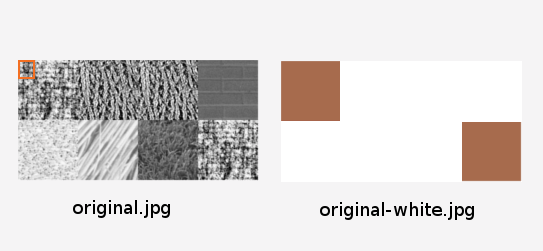
\includegraphics[width=14cm,]{Figures/chap2/4.png}
		
	\caption[coloriage1]{Coloration de la première texture détectée.}
	\label{fig:division}
\end{figure}

La recherche d'une nouvelle référence est entamée. On continu à chercher le premier carré blanc avec la même taille de références $t_r$ initialement fixée. [Figure 2.5]

\begin{figure}[H]
  \centering
    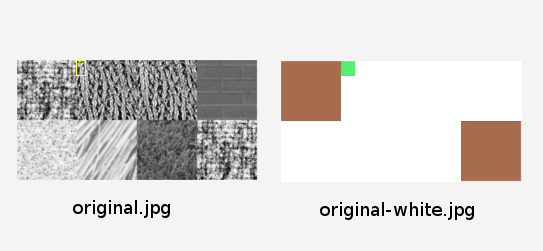
\includegraphics[width=14cm,]{Figures/chap2/5.png}
    
  \caption[detection2]{Deuxième détection.}
  \label{fig:division}
\end{figure}


Les carrés ressemblant à la nouvelle référence sont coloriés de la même façon. [Figure 2.6]

\begin{figure}[H]
  \centering
    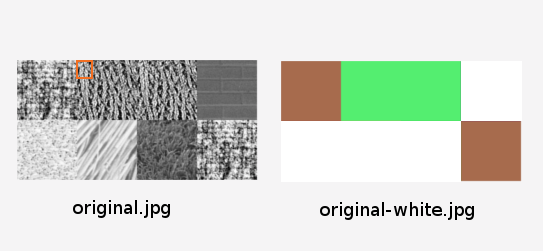
\includegraphics[width=14cm,]{Figures/chap2/6.png}
    
  \caption[coloriage2]{Coloration de la deuxième texture détectée.}
  \label{fig:division}
\end{figure}

Si aucun carré blanc de taille t ne reste dans l'IB, l'algorithme est terminé. [Figure 2.7]

\begin{figure}[H]
  \centering
    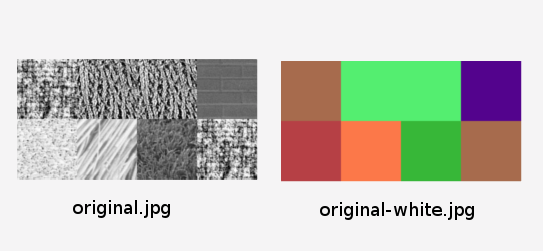
\includegraphics[width=14cm,]{Figures/chap2/7.png}
    
  \caption[coloriage]{Détection de toutes les téxtures.}
  \label{fig:division}
\end{figure}

\subsection{Variantes}
\indent Le premier problème à traiter pour une meilleure précision est de trouver le bon \textit{seuil} pour chaque texture recherchée. Et pour cela nous avons pensé à un algorithme d'apprentissage. Il s'agit d'une étape facultative. Cette dernière vise à tester d'une manière manuelle le meilleur \textit{seuil} possible pour une texture donné, et le sauvegarder dans une base de données.\\
\indent Quand vient l'étape de recherche de texture, les références seront recherchés dans la base de données suivant la ressemblance de l'histogramme sauvegardé et l'histogramme de la texture, et selon laquelle le meilleur \textit{seuil} sauvegardé sera extrait.

\subsubsection{LBP à rotation invariante }
\indent L'une des variante les plus intéressantes de la LBP est la $LBP^{riu2}$ qui est capable de détecter une texture même si cette dernière a subis une rotation d'un certain angle $\alpha$ qui est inclus dans l'ensemble suivant : $S = \lbrace 45\si{\degree}, 90\si{\degree}, 135\si{\degree}, 180\si{\degree}, 225\si{\degree}, 270\si{\degree}, 315\si{\degree} \rbrace$.\\

\indent Dans la figure 2.8, après que l'image ait subis une rotation de 45$\si{\degree}$, on remarque bien que le motif a aussi subit une rotation de 45$\si{\degree}$, mais le plus important est que le nouveau motif fait partie aussi des «\textit{uniform patterns}» tout comme le premier. 
Le motif a passé de la valeur $m=11000011$ vers la valeur $m'=11100001$.\\
De ce fait, on comprend qu'une rotation de l'image d'un angle de 45$\si{\degree}$ fait décaler les valeurs des motifs de un chiffre vers la droite, de manière générale on a :
$$ D = \frac{360\si{\degree}}{\alpha} $$
\indent La valeur du décalage $D$ dépend de la valeur de l'angle de rotation $\alpha$, et donc le choix de l'ensemble $S = \lbrace 45\si{\degree}, 90\si{\degree}, 135\si{\degree}, 180\si{\degree}, 225\si{\degree}, 270\si{\degree}, 315\si{\degree} \rbrace$ vient du fait que ce sont les seules valeurs de $\alpha$ qui donnent un nombre entier naturelle $D$ de décalage.


\begin{figure}[H]
	\centering
		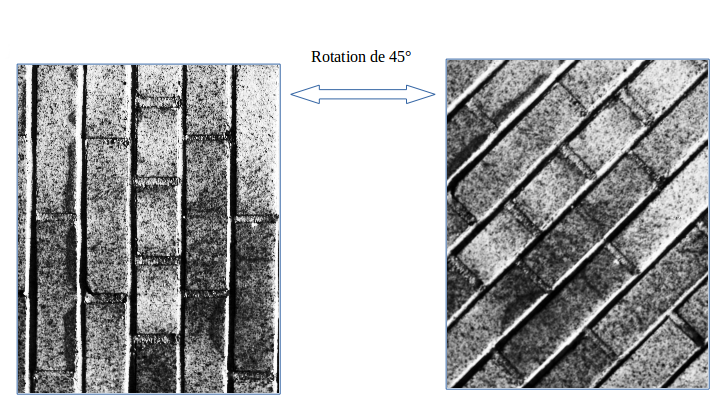
\includegraphics[width=14cm,height=8cm]{Figures/chap2/rotation45.png}
	\caption[rot1]{Un motif après une rotation de 45$\si{\degree}$}
\end{figure}


\indent Ainsi, comme chaque motif va subir un décalage de $D$ positions, et que les huit motifs résultants des huit décalages possibles, peuvent représenter toujours la même texture mais qui est sous des angles $\alpha$ différents, on peut donc regrouper les huit rotations possibles de chaque motif dans une seule valeur de l'histogramme comme le montre la figure 2.9.


\begin{figure}[H]
\centering
\begin{tabular}{cc}
\centering

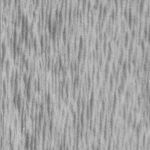
\includegraphics[width=5cm,height=4cm]{Figures/chap2/p4.png}
&
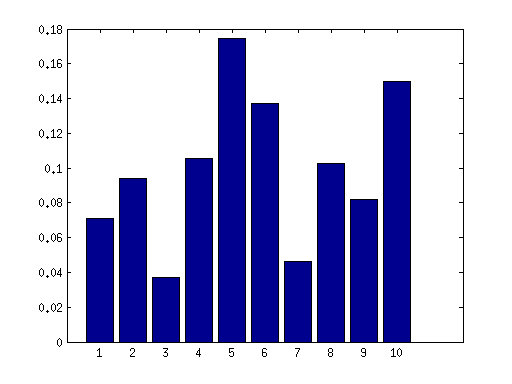
\includegraphics[width=9cm,height=4cm]{Figures/chap2/riu2a.png}\\

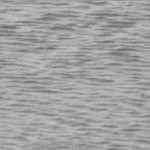
\includegraphics[width=5cm,height=4cm]{Figures/chap2/p5.png}
&
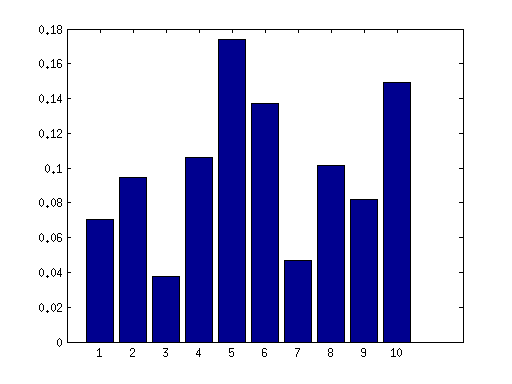
\includegraphics[width=9cm,height=4cm]{Figures/chap2/riu2b.png}\\
\end{tabular}
\caption[comp2]{Histogramme $LBP^{riu2}$ d'une texture subissant une rotation de 90$\si{\degree}$}
\end{figure}

\indent L'histogramme $LBP^{riu2}$ a dix valeurs différentes qui sont :
\begin{itemize}
\item Deux valeurs pour les motifs $m=00000000$ et $m=11111111$.
\item Sept valeurs pour les «\textit{uniform patterns}» uniques (incluant leur huit rotations) qui sont : $m=10000000$, $m=11000000$, $m=11100000$, $m=1111000$, $m=11111000$, \\
$m=11111100$, $m=11111110$.
\item Et une dernière valeur regroupant tous les «\textit{non uniform patterns}».\\
\end{itemize}

\indent On peut voir les meilleurs résultats obtenus dans la figure suivante :

\begin{figure}[H]
\centering
\begin{tabular}{cccc}
\centering

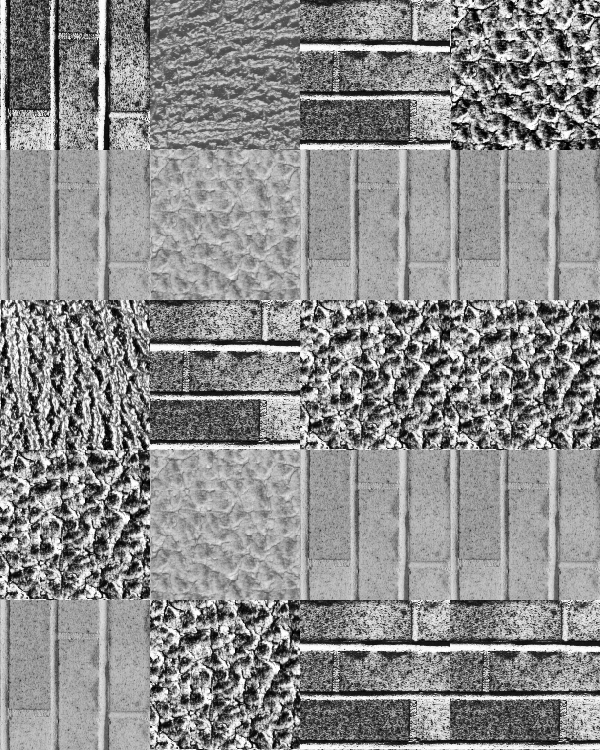
\includegraphics[width=4cm,height=4cm]{Figures/chap2/t1.png}
&

\includegraphics[width=4cm,height=4cm]{Figures/chap2/w1.png}
&
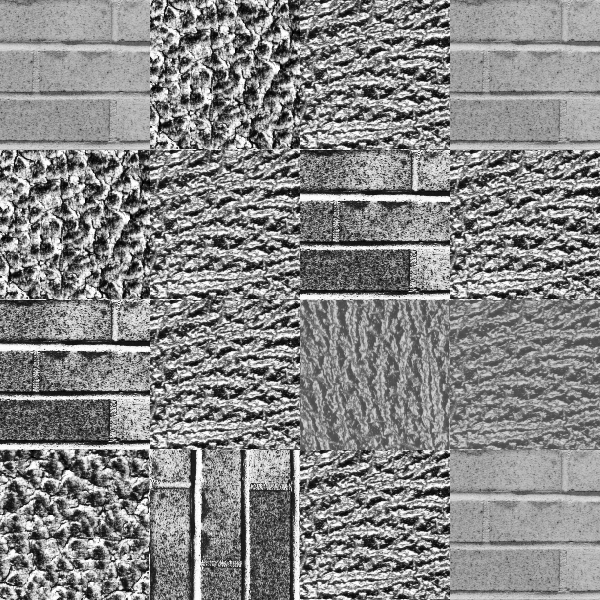
\includegraphics[width=4cm,height=4cm]{Figures/chap2/t2.png}
&

\includegraphics[width=4cm,height=4cm]{Figures/chap2/w2.png}
\end{tabular}
\caption[text3]{Segmentation avec la $LBP^{riu2}$}
\end{figure}

\indent Cependant dans certains cas, les résultats sont moins bons et cela revient au manque de précision de l'histogramme $LBP^{riu2}$, puisque chaque motif a été regroupé avec ses rotations, d'où résulte la difficulté du choix ... AJOUTER FIGURE HERE !!!!\\


\subsubsection{Segmentation par des formes circulaires}
\indent En plus de la recherche par des carrés, nous avons implémenté d'autres formes géométrique pour améliorer la détection de ces derniers.
Nous avons remarqué que, par exemple, les cercles n'étaient pas bien distingués par la méthode classique. \\
\indent Prenons l'image représentée dans la figure 2.8.

\begin{figure}[H]
	\centering
		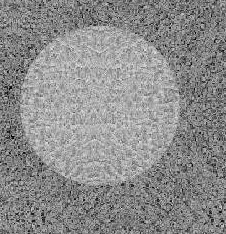
\includegraphics[width=7cm,]{Figures/chap2/8.png}
		
	\caption[img]{Image initiale.}
	\label{fig:division}
\end{figure}

La méthode classique nous a donné comme résultat l'image représenté par la figure 2.9.

\begin{figure}[H]
	\centering
		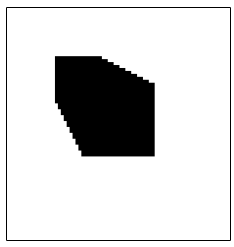
\includegraphics[width=7cm,]{Figures/chap2/9.png}
		
	\caption[imgCarre]{Détection par carrés.}
	\label{fig:division}
\end{figure}

\indent Nous avons changé la détection et le coloriage des carrés par une détection et un coloriage en cercle.\\
Nous parcourons le cercle pour créer l'histogramme et le colorier à l'aide de la formule suivante:\\
\indent Prenons le centre $O(x_0,y_0)$ du cercle \textbf{c} d'un rayon \textbf{r}.  Un pixel $P (x_p,y_p)$ fait partie du cercle si l'inéquation ci-dessous est réalisée:
$$(x_p-x_0)^2 + (y_p-y_0)^2 <= R^2$$
Nous avons eu comme résultats l'image représentée par la figure 2.10.

\begin{figure}[H]
	\centering
		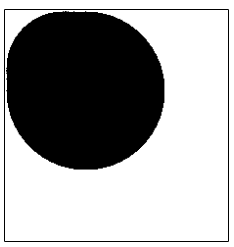
\includegraphics[width=7cm,]{Figures/chap2/10.png}
		
	\caption[imgCercle]{Détection par cercles.}
	\label{fig:division}
\end{figure}

%----------------------------------------------------------------------------------------
%	SECTION 4
%----------------------------------------------------------------------------------------

\section{Création des images de test}

\indent Les images sur lesquelles nous avons appliqué nos tests ont été généré aléatoirement. Les textures ont été tirés de la base de donnée \textit{Brodatz} [ref].

Nous avons utilisé un premier algorithme pour découper ces dernières en plus petite textures (de taille 150*150px) et les avons mis dans un dossier \textit{Textures}.

\label{algo decoupage}
\begin{algorithme}[H]
\caption{Cutting textures}
\Function{Textures' Cutting}
{\textit{Brodatz textures} : \textbf{folder}}{folder}
{
\For {Each image from \textit{Brodatz's textures}}
{
	\begin{itemize}
	\item Cut \textit{150x150} first pixels.
	\item Add the new texture to the \textit{Textures} folder
	\end{itemize}
}
\\
\Return \textit{Textures}
}
\end{algorithme}

Puis nous avons élaboré un algorithme qui sélectionne aléatoirement des textures à partir du dossier rempli précédemment et construit avec ces dernières une image à tester.

\label{algo creation}
\begin{algorithme}[H]
\caption{Création de l'image à traiter}
\Function{Create Test Image}
{\textit{Textures} : \textbf{folder}}{image}
{
Create a matrix \textit{M} of random dimensions
\For {each cell in \textit{M}}
{
	Affect a random texture from \textit{Textures}
}
\\
\textit{image} = transforming M into one image
\\
\Return \textit{image}
}
\end{algorithme}

\section{Conclusion}
\indent Nous avons présenté dans ce chapitre les détails de notre approche dans le but de segmenter les différents types de textures. Les techniques que nous avons utilisé et généralisé nous ont permis d'élaborer un programme qui détecte toutes les textures présentes sur une image quelconque, et cela d'une manière automatique.\\
\indent Les résultats des tests restent satisfaisante si nous respectons les contraintes cités au début de ce chapitre, et qui concernent la forme rectangulaire des textures recherchées. Nous avons aussi montré que d'autres formes de textures peuvent être appliquées à notre méthode afin de détecter des formes non rectangulaires.\\
\indent Nous présentons dans ce qui suit, notre application ainsi que des tests qui montreront les différents résultats obtenu à l'aide de cette méthode.
 
% Chapter Template

\chapter{Application et tests} % Main chapter title

\label{Chapter3} % Change X to a consecutive number; for referencing this chapter elsewhere, use \ref{ChapterX}


\lhead{Chapter 3. \emph{Application et tests}} % Change X to a consecutive number; this is for the header on each page - perhaps a shortened title


%----------------------------------------------------------------------------------------
%	SECTION 1
%----------------------------------------------------------------------------------------

\section{Introduction}

Nous présentons dans ce  chapitre les résultats de notre application et leur intérpertation. Ainsi que les détails des fonctionnalités disponibles.

%-----------------------------------
%	SECTION 2
%-----------------------------------
\section{Outils utilisés}

\indent Nous avons choisi comme langage de programmation le langage Python2.7 et ce pour diverses raisons dont on site [HOY 10]:\\

\begin{itemize}
\item Facilité d’écriture et de compréhension du code. On trouve moins de barrière entre la génération d'idée, et leurs traduction en code.
\item Balance entre langage de haut et de bas niveau. Ce qui forme un point fort du langage.
\item L'interopérabilité avec les autres langages, ou la capacité très utile à pouvoir appeler des script d'autres langages facilement.
\item Le grand nombre de bibliothèques disponibles.
\item La documentation abondante.\\
\end{itemize}

\indent Le traitement bas niveau des images se fait avec la bibliothèque graphique libre OpenCV qui propose un bon nombre de fonctions permettant d'effectuer les opérations classiques.\\

\indent Nous avons choisi d'utiliser pour le développement de l'interface graphique le framework PyQt, un module qui permet de lier le langage Python avec la bibliothèque Qt. En utilisant l'environnement \textit{Qt4 Designer version 4.8.1}.\\

Pour améliorer la vitesse de découpage, il s'est avéré qu'appeler un script matlab est bien plus intéressant en terme de temps d’exécution que de reprogrammer le script en python. La version de matlab utilisée étant \textit{R2012a 7.14.0.739 32-bit(glnx86)} \\

Ce document est rédigé en \textit{Latex}, avec \textit{Texmaker 3.2}.

%----------------------------------------------------------------------------------------
%	SECTION 3
%----------------------------------------------------------------------------------------
\section{Presentation et test de l'application:}

Nous commençons par exécuter l'application. [Figure 3.1]

Elle nous permet de choisir une image en cliquant sur Browse pour parcourir nos fichiers, ou en collant directement son chemin absolu.\\
Nous choisissons ensuite la valeur du \textit{threshold}.

\begin{figure}[H]
	\centering
		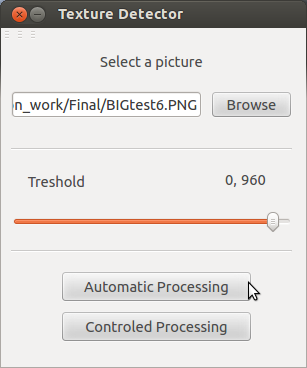
\includegraphics[width=7cm,]{Figures/chap3/3.png}
			\caption[choice1]{Fenêtre principale.}
	\label{fig:choice1}
\end{figure}

\indent Nous avons après cela le choix entre deux méthodes: 
\begin{itemize}


\item Automatic Processing: qui fait un traitement automatique des textures \\
\item Controled Processing: qui permet d'avoir plus de contrôle sur le traitement et la reconnaissance des textures. Il est aussi considéré comme processus d’entraînement de l'analyseur.\\
\end{itemize}
\indent Nous commençons par le traitement automatique. La fenêtre de la figure 3.2 nous est affiché, elle montre à droite l'image sélectionnée et en bas le \textit{threshold}, avec possibilité de les modifier.

\begin{figure}[H]
	\centering
		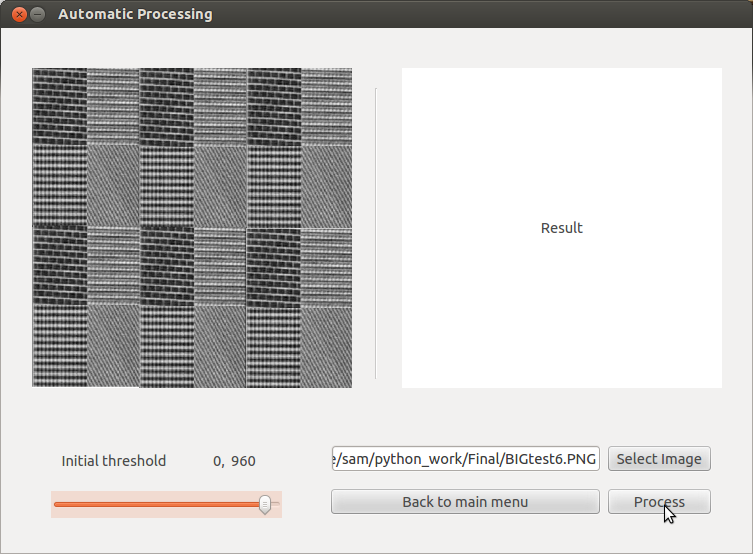
\includegraphics[width=12cm,]{Figures/chap3/4.png}
	\caption[traitementAuto]{Traitement automatique.}
	\label{fig:traitementAuto}
\end{figure}

\indent Nous cliquons sur \textit{Process} pour lancer le traitement.
Après quelques instants, le résultat de la détection et coloration des textures nous est affiché à droite de la fenêtre. [Figure 3.3]

\begin{figure}[H]
	\centering
		\includegraphics[width=12cm,]{Figures/chap3/5.jpg}
	\caption[traitementAutofin]{Traitement automatique fini.}
	\label{fig:traitementAutofin}
\end{figure}

\indent L'image résultante est automatiquement enregistrée dans le dossier contenant l'application. Comme expliqué dans le précédent chapitre, les \textit{thresholds} utilisés pour les différentes textures détectées sont tirés d'une base de données remplit à chaque usage du traitement contrôlé.

\indent Nous revenons vers le menu principale en cliquant sur le bouton \textit{Back to main menu}, et nous choisissons cette fois \textit{Controled Processing}.
Nous allons tester le traitement contrôlé où nous allons pouvoir modifier à chaque fois le \textit{threshold} de chaque texture détectée. Nous changerons aussi les informations présente dans la base de donnée en sauvegardant les résultats satisfaisants des détections d'une texture x.\\
\indent Prenons l'exemple de la figure 3.4. La première étape étant identique au traitement automatique, nous choisissons l'image et un \textit{threshold} par défaut. Nous commençons le traitement en cliquant sur \textit{Proces}.


\begin{figure}[H]
	\centering
		\includegraphics[width=15cm,]{Figures/chap3/Capture4343.png}
	\caption[traitementAutofin]{Traitement contrôlé - Itération 1.}
	\label{fig:traitementAutofin}
\end{figure}


\indent Une première texture est détectée, et les régions ressemblantes à cette dernière sont coloriées. Remarquons que le \textit{threshold} utilisé (\textit{Actual threshold 0.961}) est différent de celui choisi pour être par défaut (\textit{Initial threshold 0.960}). Ceci est du au fait que la même texture, ou une texture fortement ressemblante ai été trouvé dans la base de donnée. Le \textit{threshold} de cette dernière a été donc choisi.

\indent Nous avons, ensuite, la main pour choisir de sauvegarder le \textit{threshold} dans la base de donnée, de continuer si le résultat est satisfaisant, ou de changer ce premier et rechercher les zones ressemblantes à la texture détectée à nouveau.

\indent Nous choisissons de continuer, jusqu'a ce que l'a détection de l'une des textures n'est pas satisfaisante. Nous choisissons dans ce cas de changer le \textit{threshold}.[Figure 3.5]


\begin{figure}[H]
	\centering
		\includegraphics[width=15cm,]{Figures/chap3/Capture4826.png}
	\caption[traitementAutofin]{Traitement contrôlé - Itération 4.}
	\label{fig:traitementAutofin}
\end{figure}

Nous cliquons sur apply pour cela après avoir choisi un nouveau \textit{threshold} dans la partie \textit{Change threshold} [Figure 3.6].

\begin{figure}[H]
	\centering
		\includegraphics[width=15cm,]{Figures/chap3/Capture5010.png}
	\caption[traitementAutofin]{Traitement controlé - Itération 5.}
	\end{figure}

\indent Nous allons sauvegarder ce \textit{threshold} dans la base de donnée en appuyant sur le bouton \textit{Save} pour que la prochaine fois cette valeur sera utilisé automatiquement.

Le processus continue de la sorte jusqu’à ce que toutes les textures de l'image soient détectées [Figure 3.7].


\begin{figure}[H]
	\centering
		\includegraphics[width=15cm,]{Figures/chap3/Capture5253.png}
	\caption[traitementAutofin]{Traitement contrôlé - Itération 7.}
\end{figure}

\section{Tests et intérpretation des résultats:}

Nous allons voir plus en détails les résultats de plusieurs tests pour voir le comportement du threshold vis-à-vis des différentes textures.\\

Les détails des threshold choisi pour les textures détectés et leur surface occupé dans l'image (par carré de 150*150 px) sont représentés dans le tableau suivant .\\



%----------------- PREMIER TESTE ----------------------------------
\begin{figure}[htbp]
\centering
\begin{tabular}{cc}
\centering
\includegraphics[width=6cm,]{Figures/chap3/texture1.png}
&
\includegraphics[width=6cm,]{Figures/chap3/texture1c.png}\\
&
\end{tabular}
\caption[test1]{Test 1\\}
\end{figure}

\begin{center}
\begin{tabular}{ | c c c | }
	\hline                       
	texture & surface (par carré) & threshold\\
	\hline                       
	  1 & 2 & 0,969    \\
	  2 & 3 & 0.997  \\
	  3 & 4 & 0.973  \\
  	  4 & 2 & 0.971 \\
	  4 & 3 & 0.964\\
	  6 & 1 & 0.964 \\
	\hline                       
\end{tabular}
\end{center}

%----------------- DEUXIEME TESTE ----------------------------------

\begin{figure}[htbp]
\centering
\begin{tabular}{cc}
\centering
\includegraphics[width=6cm,]{Figures/chap3/texture2.png}
&
\includegraphics[width=6cm,]{Figures/chap3/texture2c.png}\\
&
\end{tabular}
\caption[test2]{Test 2\\}
\end{figure}

\begin{center}
\begin{tabular}{ | c c c | }
	\hline                       
	texture & surface (par carré) & threshold\\
	\hline                       
	  1 & 7 & 0,972    \\
	  2 & 4 & 0.971  \\
	  3 & 2 & 0.969  \\
  	  4 & 3 & 0.970 \\
	  5 & 1 & 0.976\\
	  6 & 2 & 0.958 \\
  	  7 & 2 & 0.973 \\
	\hline                       
\end{tabular}
\end{center}

%----------------- TROISIEME TESTE ----------------------------------

\begin{figure}[htbp]
\centering
\begin{tabular}{cc}
\centering
\includegraphics[width=6cm,]{Figures/chap3/texture3.png}
&
\includegraphics[width=6cm,]{Figures/chap3/texture3c.png}\\
&
\end{tabular}
\caption[test3]{Test 3\\}
\end{figure}

\begin{center}
\begin{tabular}{ | c c c | }
	\hline                       
	texture & surface (par carré) & threshold\\
	\hline                       
	  1 & 7 & 0,972    \\
	  2 & 4 & 0.972  \\
	  3 & 2 & 0.965  \\
  	  4 & 4 & 0.958 \\
	  5 & 3 & 0.973\\
	\hline                       
\end{tabular}
\end{center}


%-------------------- MOYENNE -------------------------

\paragraph*{}
Nous avons fait une dizaine de tests similaires. Nous avons calculé les moyenne des treshold par image dans un premier lieu, et puis, nous avons pris en compte les coefficients en fonction de la surface qu'ils occupent dans l'image. \\

Les résultats sont représentés dans le graphe suivant:

Graph représentatifs des moyenes.

\paragraph*{}
Nous remarquons que, malgré la différence considérable entre les thresholds des différentes textures, la moyenne entre ces derniers restes constante. Et ce, que ce soit avec ou sans compter le coéfficient relative à la surface occupée par les textures. 

Ceci implique que la précision en terme de détection reste élevée.


\subsection{Tests suplémentaires}

\begin{figure}

\begin{tabular}{cccc}


\multicolumn{2}{c}{\includegraphics[width=8cm, height=4cm]{Figures/chap3/cercle1.png}}
&
\multicolumn{2}{c}{\includegraphics[width=8cm, height=4cm]{Figures/chap3/cercle1cc.png}}\\

\multicolumn{4}{c}{(a) Image avec cercle}\\


\multicolumn{2}{c}{\includegraphics[width=8cm, height=4cm]{Figures/chap3/randome1.png}}
&
\multicolumn{2}{c}{\includegraphics[width=8cm, height=4cm]{Figures/chap3/randome1cc.png}}\\

\multicolumn{4}{c}{(b) Image aléatoire 1}\\


\includegraphics[width=4cm, height=4cm]{Figures/chap3/first.png}
&
\includegraphics[width=4cm, height=4cm]{Figures/chap3/first2.png}
&
\includegraphics[width=4cm, height=4cm]{Figures/chap3/second.png}
&
\includegraphics[width=4cm, height=4cm]{Figures/chap3/second2.png}\\

\multicolumn{2}{c}{(c) Image aléatoire 2}
&
\multicolumn{2}{c}{(d) Image aléatoire 3}\\


\includegraphics[width=4cm, height=4cm]{Figures/chap3/port1.jpg}
&
\includegraphics[width=4cm, height=4cm]{Figures/chap3/san_fransisco2.png}
&
\includegraphics[width=4cm, height=4cm]{Figures/chap3/port1.jpg}
&
\includegraphics[width=4cm, height=4cm]{Figures/chap3/san_fransisco2.png}\\

\multicolumn{2}{c}{(c) San Fransisco}
&
\multicolumn{2}{c}{(d) Image aléatoire 2}

\end{tabular}
\caption[TraitementImage]{La segmentation d'images}

\end{figure}

\section{Conclusion}
\indent Dans ce dernier chapitre nous avons décrit l'interface de notre application et les détails de son fonctionnement. Nous avons fait une démonstration des deux différents modes d'utilisation : \textbf{automatique} et \textbf{contrôlé} (étape d'apprentissage) et avons aussi exposé les multiples options proposées dans ce dernier mode.\\
\indent Nous avons présenté une série de tests effectués sur différentes images aléatoirement construites et qui donnent des résultats satisfaisants et très prometteurs.\\
\indent Enfin, nous avons vu l'indépendance de cette méthode des formes utilisées pour la recherche et la reconnaissance des textures, qui représente un très grand avantage.


% Chapter 4
\chapter*{Conclusion générale}

\label{Chapter4} % Change X to a consecutive number; for referencing this chapter elsewhere, use \ref{ChapterX}

\lhead{\emph{Introduction générale}} % Change X to a consecutive number; this is for the header on each page - perhaps a shortened title

%------------------------------------------------------------------------------
%	INTRODUCTION GENERALE
%----------------------------------------------------------------------------------------

\paragraph*{}
Nous avons parcouru, tout au long de ce mémoire, les différentes étapes de la segmentation d'image basées sur la méthode de reconnaissance de texture, et nous pouvons dire que ce travail démontre la puissance de cette dernière.

\paragraph*{}
Nous avons étudié les aspects statistiques de la caractérisation des textures, et plus précisement, la caractéristique LBP qui nous a offert un outils de reconaissance très puissant. Nous avons aussi étudié la méthode de segmentation dynamique qui permet de détecter une texture donnée, dans une image donnée, 
Notre travail consistait à élaborer une méthode de généralisation pour la détection automatique de toutes les textures présentes dans une image, sans avoir, au préalable, aucune information à part l'image elle même.
Les résultats obtenu restent très prometteurs et motivants pour accorder à cette étude plus de temps et d'efforts. 

\paragraph*{}
Bien que certaines contraintes ont du être respectés, il faut savoir que ce travail est une première étape d'application de cette méthode. Néomoin, nous aurions souhaité bénificier de plus de temps pour mettre en application nos idée qui consistent à, premièrement, lier la reconnaissance et la segmentation de texture à des descriptions dans un format compréhensible par une machine. Celle ci, pourrait très bien comprendre si elle est en train de survoler une zone forestière ou urbaine. 

\paragraph*{}
Aussi, pour trouver un accord entre les différentes formes géométriques pour la détection des textures, nous pensons on continuer avec une reconnaissance de formes régulières. Ce travail peut-etre enrichi en implémentant l'algorithme avec des formes hexagonales. 
Ces formes représentent, théoriquement, un très bon compromis entre les différentes autres formes. Leur nature permet d'englober uniformément une surface entière tout en évitant les chevauchements (contrairement aux cercles, par exemple). Son avantage par rapport aux formes carrées et aux triangles équilatérales est le fait qu'un hexagone couvre bien plus efficacement une surface ronde. En effet, le rapport entre la surface d'un triangle équilatéral et un cercle est de 17.77\%. Celle d'un carré est de 63.7\%. En fin, celle d'un hexagone n'est pas moins de 83\%.

\paragraph*{}
Nous avons décidé de continuer personellement ce travail afin d'aboutire à d'autres résultats souhaités.

%----------------------------------------------------------------------------------------




%\bibliography{bib}

%\clearpage % Start a new page
\end{document}